% IEEE Paper Template for A4 Page Size (V1)
% Sample Conference Paper using IEEE LaTeX style file for A4 pagesize.
% Copyright (C) 2006-2008 Causal Productions Pty Ltd.
% Permission is granted to distribute and revise this file provided that
% this header remains intact.
%
% REVISION HISTORY
% 20080211 changed some space characters in the title-author block
%
\documentclass[a4paper]{spie}

\usepackage[utf8]{inputenc}
\usepackage{fontenc}
\usepackage[T1]{fontenc}
\usepackage{url}
\usepackage{multirow}
\usepackage{multicol}
\usepackage{algorithm}
\usepackage{algpseudocode}
\usepackage{graphicx}
\usepackage{import}
\usepackage{xcolor}
\usepackage{amsmath}
\usepackage{amsfonts}
\usepackage{amssymb}
%\usepackage{amsthm}
\usepackage{natbib}

\newcommand{\chg}[1]{{\color{blue} #1}}
\newcommand{\todo}[1]{{\color{red} TODO: #1}}

\setcitestyle{numbers,square}

%% \usepackage{lineno}
%% \pagewiselinenumbers


\title{WebOmics as a tool to view and explore genomic data}

\author{Michał Haponiuk$^{1}$, Magdalena Pawełkowicz$^{2}$, Robert Nowak$^{1}$, Zbigniew Przybecki$^{2}$
  \skiplinehalf
  $^{1}$ Institute of Computer Science, Warsaw University of Technology; Nowowiejska 15/19, 00-665, Warsaw, Poland\\
  $^{2}$ Department of Plant Genetics, Breeding and Biotechnology, Warsaw University of Life Sciences; Nowoursynowska 159, 02-776, Warsaw, Poland\\
}

\authorinfo{Further author information: (Send correspondence to Robert Nowak)\\
  Robert Nowak: E-mail: r.m.nowak@elka.pw.edu.pl}

\begin{document}
\maketitle

\begin{abstract}
  Integrated WebOmics is an easy-to-use, open-source, on-line tool that can be used to browse, analyze,
  and query genomic data and annotations.
  It places annotation tracks beneath genome coordinate positions, allowing rapid visual correlation of different types of information.
  It also allows users to upload and display their own experimental results or annotation sets.
  An important functionality of the application is a possibility to find similarity between sequences by applying four different algorithms of different accuracy.
  The presented tool was tested on real genomic data and is extensively used by Polish Consortium of Cucumber Genome Sequencing.
\end{abstract}

\keywords{web application, genomic viewer, similarity finding, annotation, contig, scaffold}

\section{Introduction}

We now live in the post genomic era, where it is simple to decode and access entire genomes.
The goal of computational biology and bioinformatics is to provide computer-based methods for coping with and interpreting the genomic data
that is being uncovered in large volumes within the diverse genome sequencing projects and other new experimental technologies in molecular biology.
There is a strong demand for immediate solutions in the field,
because the uncovered genomic data encode many biological insights whose deciphering can be the basis for scientific and economic success.
Large data sets are produced day by day, by the sequencing technology of genomes,
therefore the requirements to handle and manage such data are apparent.

Genome browser provides a graphical interface for users to browse, search, retrieve and analyze genomic sequence and annotation data.
Here we present the new tool -- WebOmics (WO).
We attempt to give an overview of the main functions and features of this web-based tool,
covering data visualization, retrieval, analysis and customization.
To give a brief introduction to our computer program, we describe the user interface and the most important features
using the North European cucumber genome \cite{woycicki2011genome} as an example.
The user guide with 'getting started' section and installation instructions is available at project website.

\section{Software functionality}

WebOmics (WO) is a genome browser tool for visualizing and manually annotating whole genomes.
This tool provides:
\begin{itemize}
\itemsep0em
\item display of sequence and annotation tracks;
\item interactive zoom from megabase to nucleotide resolution;
\item editing of individual features, supporting manual annotation;
\item intuitive aligned sequences, elegant to view;
\item an option for being run as online client-server as well as standalone application;
\item the possibility to integrate physical and genetic maps.
\end{itemize}

Though other genome browsers, listed in Tab.~\ref{tab:comparison}, with similar feature sets exist,
we believe that the presented application provides a more flexible and intuitive user interface.
This software is available at \url{http://webomics.sourceforge.net} under GNU Library or Lesser General Public License version 2.0 (LGPLv2).
The source code is open, the users with programming experience could modify and customize our application.

WO is platform portable, can be installed on any modern operating system (Microsoft Windows, Linux, BSD, OSx, etc.).
It was tested in Microsoft Windows 7 and Ubuntu 12.10.
No Unix or scripting knowledge is required so it is easily accessible to the average biologist with little computing experience.
The presentation layer is deployed on web browser, therefore the computer program is available for many platforms (PC, tablets, smartphones).
The graphical user interface (GUI) permits images to be drawn with minimal user input,
yet allows highly customizable figures to be generated for closer analysis or even publication.
WO accepts multiple sequences with or without annotation in standard formats (i.e. FASTA or CSV).
The input DNA sequence is rendered to scale as a solid black line centered vertically.
The presented computer program can handle a variety of sequences lengths, from full chromosome or scaffolds  (Fig. \ref{fig:organism})
to individual loci or genes (Fig. \ref{fig:chromosome}).
The relative orientation of each region (forward/reverse) can be specified so that input sequences can be ‘flipped’ if required.

WO produces an image showing genome and components such as: contigs, coding sequences, markers and many others.
The user can specify an additional feature bond to specific position and/or specific region.
User-specified features connected with coloring scheme could be used to filter and to highlight interesting places or interesting regions.
Visualized genomic regions can be zoomed in and out, and scrolled left or right.
A ‘zoom’ feature enables subregions of large sequence files to be examined in more detail.

\begin{figure}[htp]
  \centering
  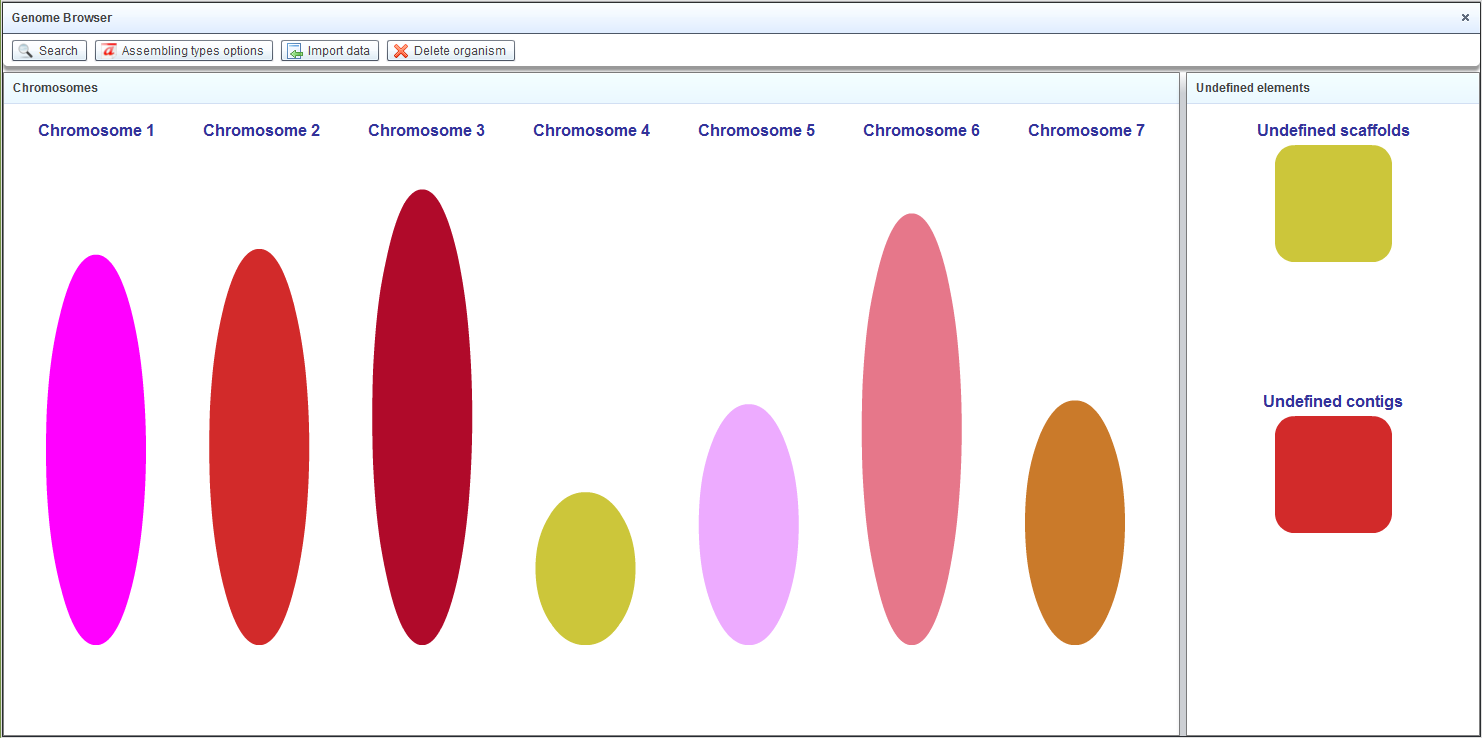
\includegraphics[width=0.7\textwidth]{img/organism.png}
  \caption{User interface main window with cucumber chromosomes}
  \label{fig:organism}
\end{figure}


\begin{figure}[htp]
  \centering
  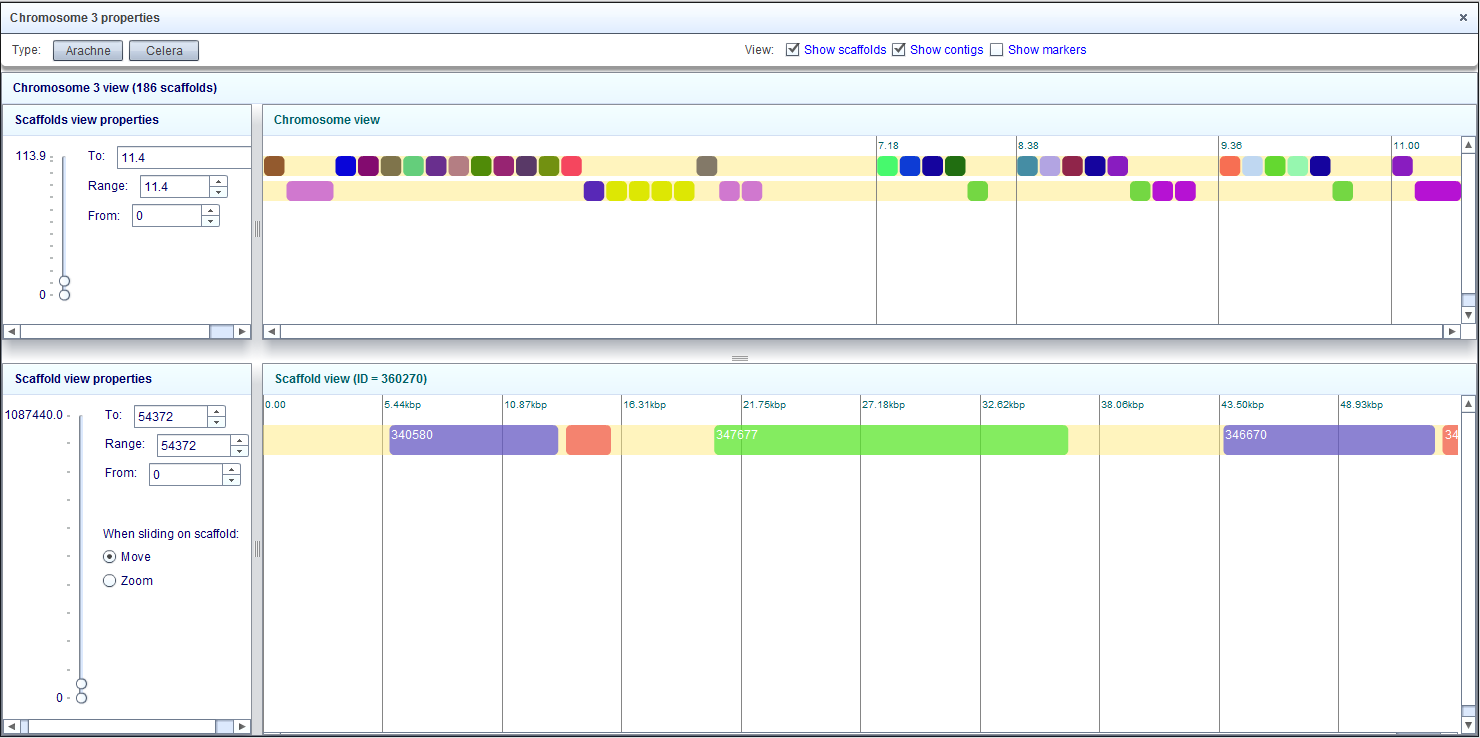
\includegraphics[width=0.7\textwidth]{img/chromosome.png}
  \caption{Detailed description of third chromosome in working window}
  \label{fig:chromosome}
\end{figure}



\section{Architecture and implementation details}

\subsection{Architecture}

The client--server architecture was chosen to obtain high performance, the software flexibility,
its availability from a~web browser and the simplified software update.
The bioweb framework was used \cite{rn:bmri2014biosoftarch},
therefore the application is deployed on client machine (presentation layer) and on server machine (time consuming algorithms, database).
The application modules with specified interfaces are used as depicted in Fig.\ref{fig:architecture}.

The data is stored in general purpose database management system PostgreSQL.
Communication with others modules is carried out through Django Object Relational Mapping,
therefore usage of other DBMS (MySQL, SqlLite, Oracle, MsSQL etc.) is possible.
The PostgreSQL provides efficient data storage with a mechanism for the transactions.

The logic layer, responsible for data processing, involves the modules implemented in C++ and in Python.
The C++ modules include the calculation algorithms that require most computer power,
e.g. custom implementation of BLAST \cite{altschul1997gapped}, Smith-Waterman \cite{smith1981identification}, Knuth-Morris-Pratt \cite{knuth1977fast}
and Boyer-Moore \cite{boyer1977fast} methods.
The C++11 concurrency mechanism applied here speeds-up the computations in multi-core and multi-processor environment.
Communication with Django web application framework is provided by Boost.Python wrappers \cite{rn:cpp}.
The BioPython library is here a collection of reference algorithms and it is used to test and to compare our implementation.

The presentation layer uses a web browser (as in thin client applications), but the Adobe Flash plugin is required.
The client partly processes information, e.g. validates user input, generates pictures to decrease the server and network load.
The client application is asynchronous -- can send and retrieve data in the background, like the Asynchronous JavaScript and XML (AJAX) techniques.
The Apache Flex Software Development Kit is the main technology involved in creating the client modules.

The client and server machines could be physically separated by the Internet or intranet,
because the standard HTTP server (Lighttpd or Apache) is used.
The messages are encapsulated of the payload in the AMF and further in HTTP format.
This will allow the data to pass through any network elements, including firewalls and address translations.

All modules are portable and could work in different operating systems and processor architectures, and only the C++ modules require the source code rebuilding.
The used libraries have non-restrictive licenses and could be used in commercial and free software.

\begin{figure}[htp]
  \centering
  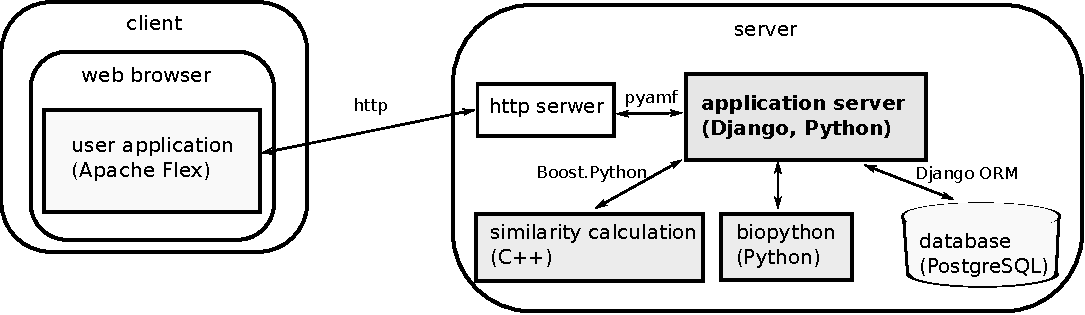
\includegraphics[width=0.7\textwidth]{img/wov_architecture.pdf}
  \caption{Modules and its interfaces in WO application.
    Persistence and logic layers are deployed on server site, the presentation layer is deployed on client machine.
    All modules are portable.}
  \label{fig:architecture}
\end{figure}

\subsection{Similarity algorithms}

An important functionality of the WO are sequence alignment algorithms, search algorithms patterns and graphic display of alignment results.
These algorithms are particularly  applicable in matching unknown fragments of the genome sequence.
The application user has the opportunity to select one of four comparison methods: BLAST, Smith-Waterman, Knuth-Morris-Pratt and Boyer-Moore.
The example, BLAST with Smith-Waterman searching, is depicted in~Fig.~\ref{fig:search}.


\begin{figure}[htp]
  \centering
  \begin{tabular}{ll}
    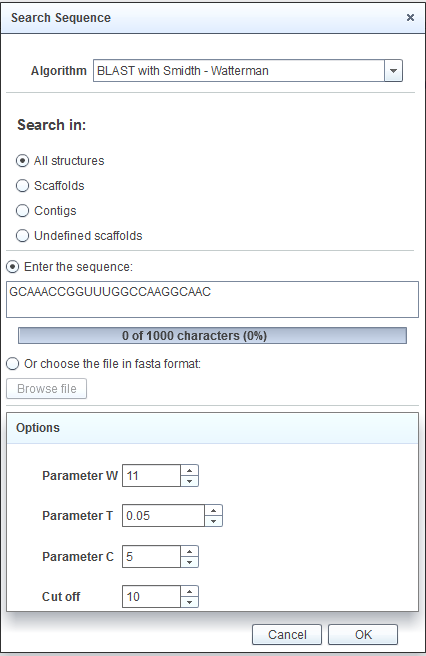
\includegraphics[width=0.35\textwidth]{img/search_similar_blast_sw.png}
    &
    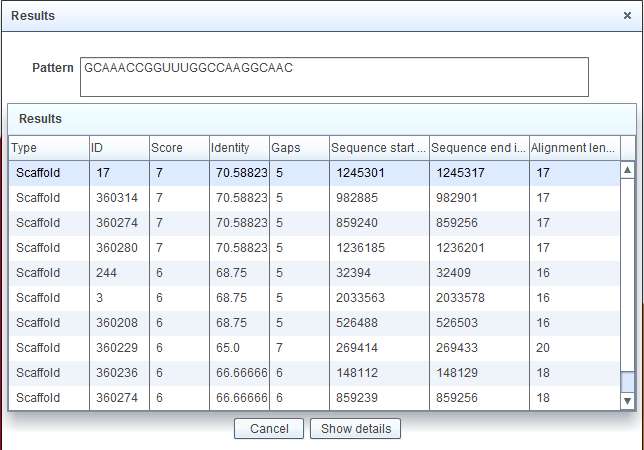
\includegraphics[width=0.35\textwidth]{img/search_similar_results.png}
  \end{tabular}
  \caption{The search for sequence using BLAST and Smith-Waterman algorithm (on left) and search results (on right).}
  \label{fig:search}
\end{figure}

BLAST is most widely used, heuristic algorithm, to search for similar regions in sequences.
WO allows customization of the minimum expect values, lengths and identities of BLAST hit to be displayed in the image.
Additionally, comparisons between two or more loci and use of previously generated tabular comparison files (converted to BLAST hit table format) is available.
The compared regions can also be rolled left, right or centered to their best BLAST hit, the hits are coloured on a gradient according to the BLAST identity value.
The colour scheme of the alignment can also be defined by the user.

In order to increase the BLAST efficiency, the Smith-Waterman algorithm is used at final step, with the highest similarity according to the BLAST.
The purpose (of this) is to examine the measures that are accurate alignment for the selected best matches.

The Knuth-Morris-Pratt is a linear time complexity algorithm to search for exact matching of strings, as well as the Boyer-Moore algorithm.
The last one is better in string benchmark, because it preprocesses the string being searched for, but not the string being searched in.
It is thus well-suited for applications in which the pattern is much shorter than the text or does persist across multiple searches.

The presented algorithms could be used for various analyzes and examinations.
In our opinion the Knuth-Morris-Pratt or/and Boyer-Moore can serve as a tool to find identical sequences
at the sequence of source or locate recurring subsequence.
The Smith-Waterman has higher time complexity, but it is accurate and includes mismatches(i.e., insertions and deletions).
The BLAST, as a representative of heuristic algorithms, is particularly useful for rapid cognition willingness highly similar sequences.

\section{Discussion}

Rapid development of sequencing technologies, increasing in effectiveness and simultaneously lowering the costs, resulted in genomes massive sequencing. The number of assembled genomes almost doubles each year.
Beside information about the order of nucleotides,
DNA sequence becomes a source of data for further steps like structural and functional annotation, polymorphisms discovery and markers detection.
The transcriptoms sequencing projects extend genetic databases even more.
In this vast accumulation of information,
a simple and clear way of visualization, access and modification of data is necessary.
Since early 2000s the web based browsers for genomic purposes have been developed.
Simultaneously, several large projects for genomic data integration and browsers implementations were executed
resulting in Ensembl \cite{hubbard2002ensembl}, UCSC \cite{karolchik2003ucsc} and Gremene \cite{ware2002gramene} web platforms.
They were started as free online services with implemented genomic and transcriptomic databases from one or many species,
enabling simplified data mining features.
Subsequently, some of them provided browsers framework.
At the same time, a framework for local usage by scientists was constructed by Generic Model Organism Database (GMOD) project \cite{stein2002generic}.
It enabled every research group to convert FASTA files and tabular data into easily accessible, interactive web page with embedded bioinformatics tools.

WO (WO) was developed due to two main factors: rapidly expanding genomic database of Northern European cucumber, containing massive amounts of data,
separated in several not integrated sections impeded information access and transparency.
Secondly, most popular framework for local installation and creation genomic browsers GBrowse is based on static web pages and
does not provide smooth interactive browsing like frameworks based on modern technologies.

Our software is a web based framework for storage and management of massive genomic, transcriptomic and proteomic data.
Configuration and format of introduced information has been simplified versus most programs allowing for smoother and swifter start up for new species or varieties.
Currently, one species application is functional with a goal for multispecies genome comparisons like  Ensembl and UCSC as depicted in Tab.~\ref{tab:comparison},
however it is possible to input several genomes data for independent browsing  but without interaction mode.
The most important feature provided by all available browsers and WO is data input and comparison executed by end users through the user interface.
This function is essential for genomic and transcriptomic information sharing with others research teams.
Contrary to Alamut \url{http://www.interactive-biosoftware.com/}, Celera Genome Browser \url{http://sourceforge.net/projects/celeragb/}
and Vista \cite{visel2007vista}, WO implemented as a web browser becomes a universal tool accessible for different devices ranging from personal computers,
tablets to smartphones and compatible with both windows and UNIX based systems.
Similarly to the most developed AJAX-based JBrowse \cite{skinner2009jbrowse}, ABrowse \cite{kong2012abrowse} and Anno-J \cite{lister2008highly}
WO provides full interactive access to genomic data with smooth scanning throughout the whole genome,
exhibiting nucleotide sequence, structural annotation and functions of annotated genes.
Being also stand-alone framework WO can be used as a data sharing tool for sensitive information
among researchers from one department or institution as opposed to genome browsers implemented only for online operation.
WO like most browser supports search function; however, this browser exploits three different algorithms including BLAST,
which is not implemented in several modern browsers: Synbrowse \cite{pan2005synbrowse}, GeneWall \url{http://www.wobblebase.com/GeneWall},
Celera Genome Browser.
This results in more accurate and precise outcome of new genes, regulatory elements and markers localization in genome and identifying homologous
from different varieties and species.
Main processes are carried out on  high power server with a broadband internet connection,
where all databases are present and every inquiry from client is analyzed and elaborated providing fast and high quality service
even for end users with low computational power.

\begin{table}

  \centering

  \begin{tabular}{|l|c|c|c|c|c|c|c|c|c|p{1cm}|p{1cm}|} \hline
    ~ & Embedded & \multicolumn{2}{|c|}{Custom species}
    & \multicolumn{3}{|c|}{Searching} & Frame- & Stand & Mobile \\
    ~ & data & one & many
    & BLAST & SW & KMP & work & -alone & devices \\ \hline
    Ensembl               & + & + & + &  + & - & - &  + &+ & +  \\ \hline
    UCSC                  & + & + & + &  + & - & - &  + &+ & +  \\ \hline
    Gramene               & + & + & + &  + & - & - &  - &- & +  \\ \hline
    Gbrowse               & - & + & + &  + & - & - &  + &+ & +  \\ \hline
    Jbrowse               & - & + & + &  + & - & - &  + &+ & +  \\ \hline
    Abrowse               & - & + & + &  + & - & - &  + &+ & +  \\ \hline
    Anno-J                & - & + & + &  + & - & - &  + &+ & +  \\ \hline
    SynBrowse             & - & + & + &  - & - & - &  + &+ & -  \\ \hline
    SynView               & - & + & + &  - & - & - &  + &+ & +  \\ \hline
    LookSeq               & - & + & + &  + & - & - &  + &+ & +  \\ \hline
    Vista                 & + & - & - &  + & - & - &  - &- & -  \\ \hline
    Celera Genome Browser & - & + & - &  - & ND& ND&  + &+ & -  \\ \hline
    Alamut                & +*& - & - &  + & ND& ND&  - &- & -  \\ \hline
    GeneWall              & +*& - & - &  - & - & - &  - &+ & +  \\ \hline
    GenomeView            & - & + & + &  + & - & - &  + &+ & -  \\ \hline
    \textbf{WebOmics}     & - & + & + &  + & + & + &  + &+ & +  \\ \hline
  \end{tabular}

  \caption{Genome browsers functionality comparison; Embedded data -- online service with embedded data,
    Custom Species -- ability to add user data on one or many species,
    SW -- Smith-Waterman algorithm, KMP -- Knuth-Morris-Pratt algorithm,
    Framework -- ability to install software on user server, Stand-alone -- ability to install software on PC without Internet access,
    ND -- no data, * -- only human database}
  \label{tab:comparison}

\end{table}

\section{Conclusion}

The WebOmics implements most modern solutions for managing genomic resources obtained through new generation sequencing,
structural and functional annotation and more.
User friendly interface enables fast and effective data search.
Genomic and annotation data exhibit in WO provides a different view on it contrary to tabular management, especially with North European Cucumber.
Embedded tools extended by internet access even in stand-alone distribution simplify the work of a researcher,
who can focus on results rather then on analysis processes.
This instrument allows for swift information exchange with other research institution with a possibility of restricting sensitive date to your department.
Further development of WebOmics will be implemented to keep up with genomic and transcriptomic massive data analysis.

\section*{Acknowledgements}

This work was supported by grants from National Science Center 2011/01/B/NZ2/01631 and N N302083139
and the statutory research of Institute of Electronic Systems of Warsaw University of Technology.

\bibliographystyle{unsrt}
\bibliography{webomics.bib}

\end{document}
